\section{Introduction}
Zcash represents a particularly interesting and innovative cryptocurrency with a number of unique features that differentiate it from other virtual currencies currently in circulation. Unlike most cryptocurrencies, which publicly reveal full transaction history on a distributed ledger, Zcash offers significant added value in terms of confidentiality, enhancing user privacy through advanced cryptographic techniques.

\noindent Zcash is the first completely open source cryptocurrency that comprehensively protects transactional privacy. This is achieved through the use of \textbf{ZKP (Zero-Knowledge Proofs)} technology, which prevents the reconstruction of asset passages, keeping transactions anonymous.

\noindent The creation of Zcash is the result of the work of a team of security engineers who developed an open source platform based on a modified version of the code of \textbf{Bitcoin}. The team includes almost all the creators of the Zerocoin and Zerocash protocols, a combination of scientists, engineers and consultants with advanced skills in cryptography and computer security.

\noindent Zcash originated in 2013 as \textbf{Zerocoin}, a project initiated by a group of researchers at Johns Hopkins University, including Matthew Green, Ian Miers, Christina Garman and Aviel D. Rubin. The main goal was to address the lack of privacy in Bitcoin by developing a cryptographic extension that would allow completely anonymous transactions. Zerocoin, initially conceived as an enhancement for Bitcoin, evolved in 2014 into \textbf{Zerocash}, a stand-alone digital currency that hides not only the origin of transactions but also the amount transferred.

\noindent Zcash was officially launched on 28 October 2016, distinguished by its use of \textbf{zk-SNARK (Zero-Knowledge Succinct Non-Interactive Argument of Knowledge)}, a cryptographic technology that allows transactions to be verified without revealing private details such as the sender, recipient or amount. This innovation allows Zcash to offer a higher level of privacy than Bitcoin, as sensitive information remains encrypted and invisible even on a public blockchain.

\noindent A useful analogy to understand the difference between Bitcoin and Zcash is that between the HTTP and HTTPS protocols. While HTTP is a protocol with no security guarantees, HTTPS adds a layer of protection based on encryption. Similarly, Zcash enhances the security and anonymity of transactions on a blockchain architecture similar to that of Bitcoin.

\noindent Zcash users can choose the degree of transparency of their transactions, opting for transparent or protected transactions via zk-SNARK. Zcash also offers features such as \textit{display keys} and \textit{payment disclosure}, which allow transaction details to be revealed only when necessary.

\noindent Despite its advanced privacy capabilities, it has been observed that many users prefer transparent transactions, limiting the effectiveness of Zcash's privacy features. This trend highlights the need for further studies and improvements to the protocol to maximise the privacy benefits offered by Zcash.

\noindent For a more detailed view of the history of Zcash see Figure \ref{fig:timeline}, which illustrates key historical events such as the founding of Zcash in 2016, the activation of the Overwinter and Sapling protocols, and the first halving in 2020. The current roadmap, which looks ahead to 2024, includes supporting the features introduced in Zcash, researching a PoW-PoS hybrid consensus model, and developing products to foster Zcash adoption.

\begin{figure}[!ht]
    \centering
    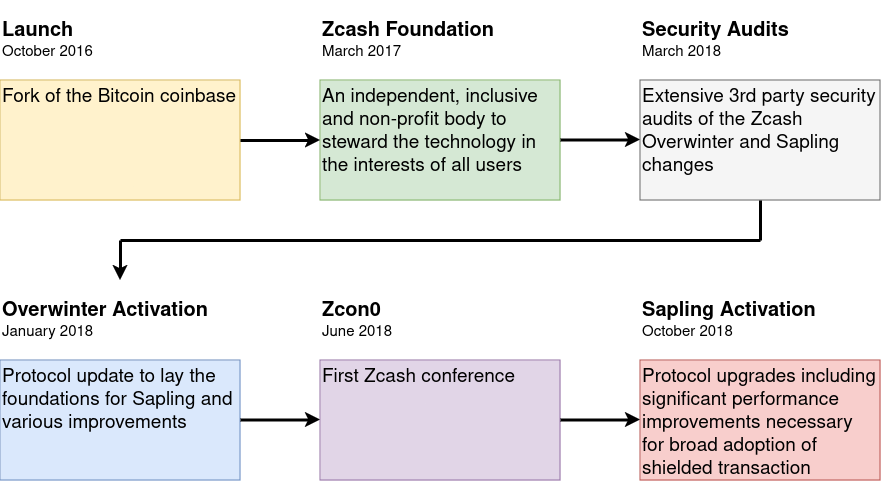
\includegraphics[width=1\linewidth]{img/timeline.png}
    \caption{Zcash Community History \cite{youtube}}
    \label{fig:timeline}
\end{figure}